\section{Implementación}\label{sec:implementacion}

\begin{figure}[H]
    \centering
    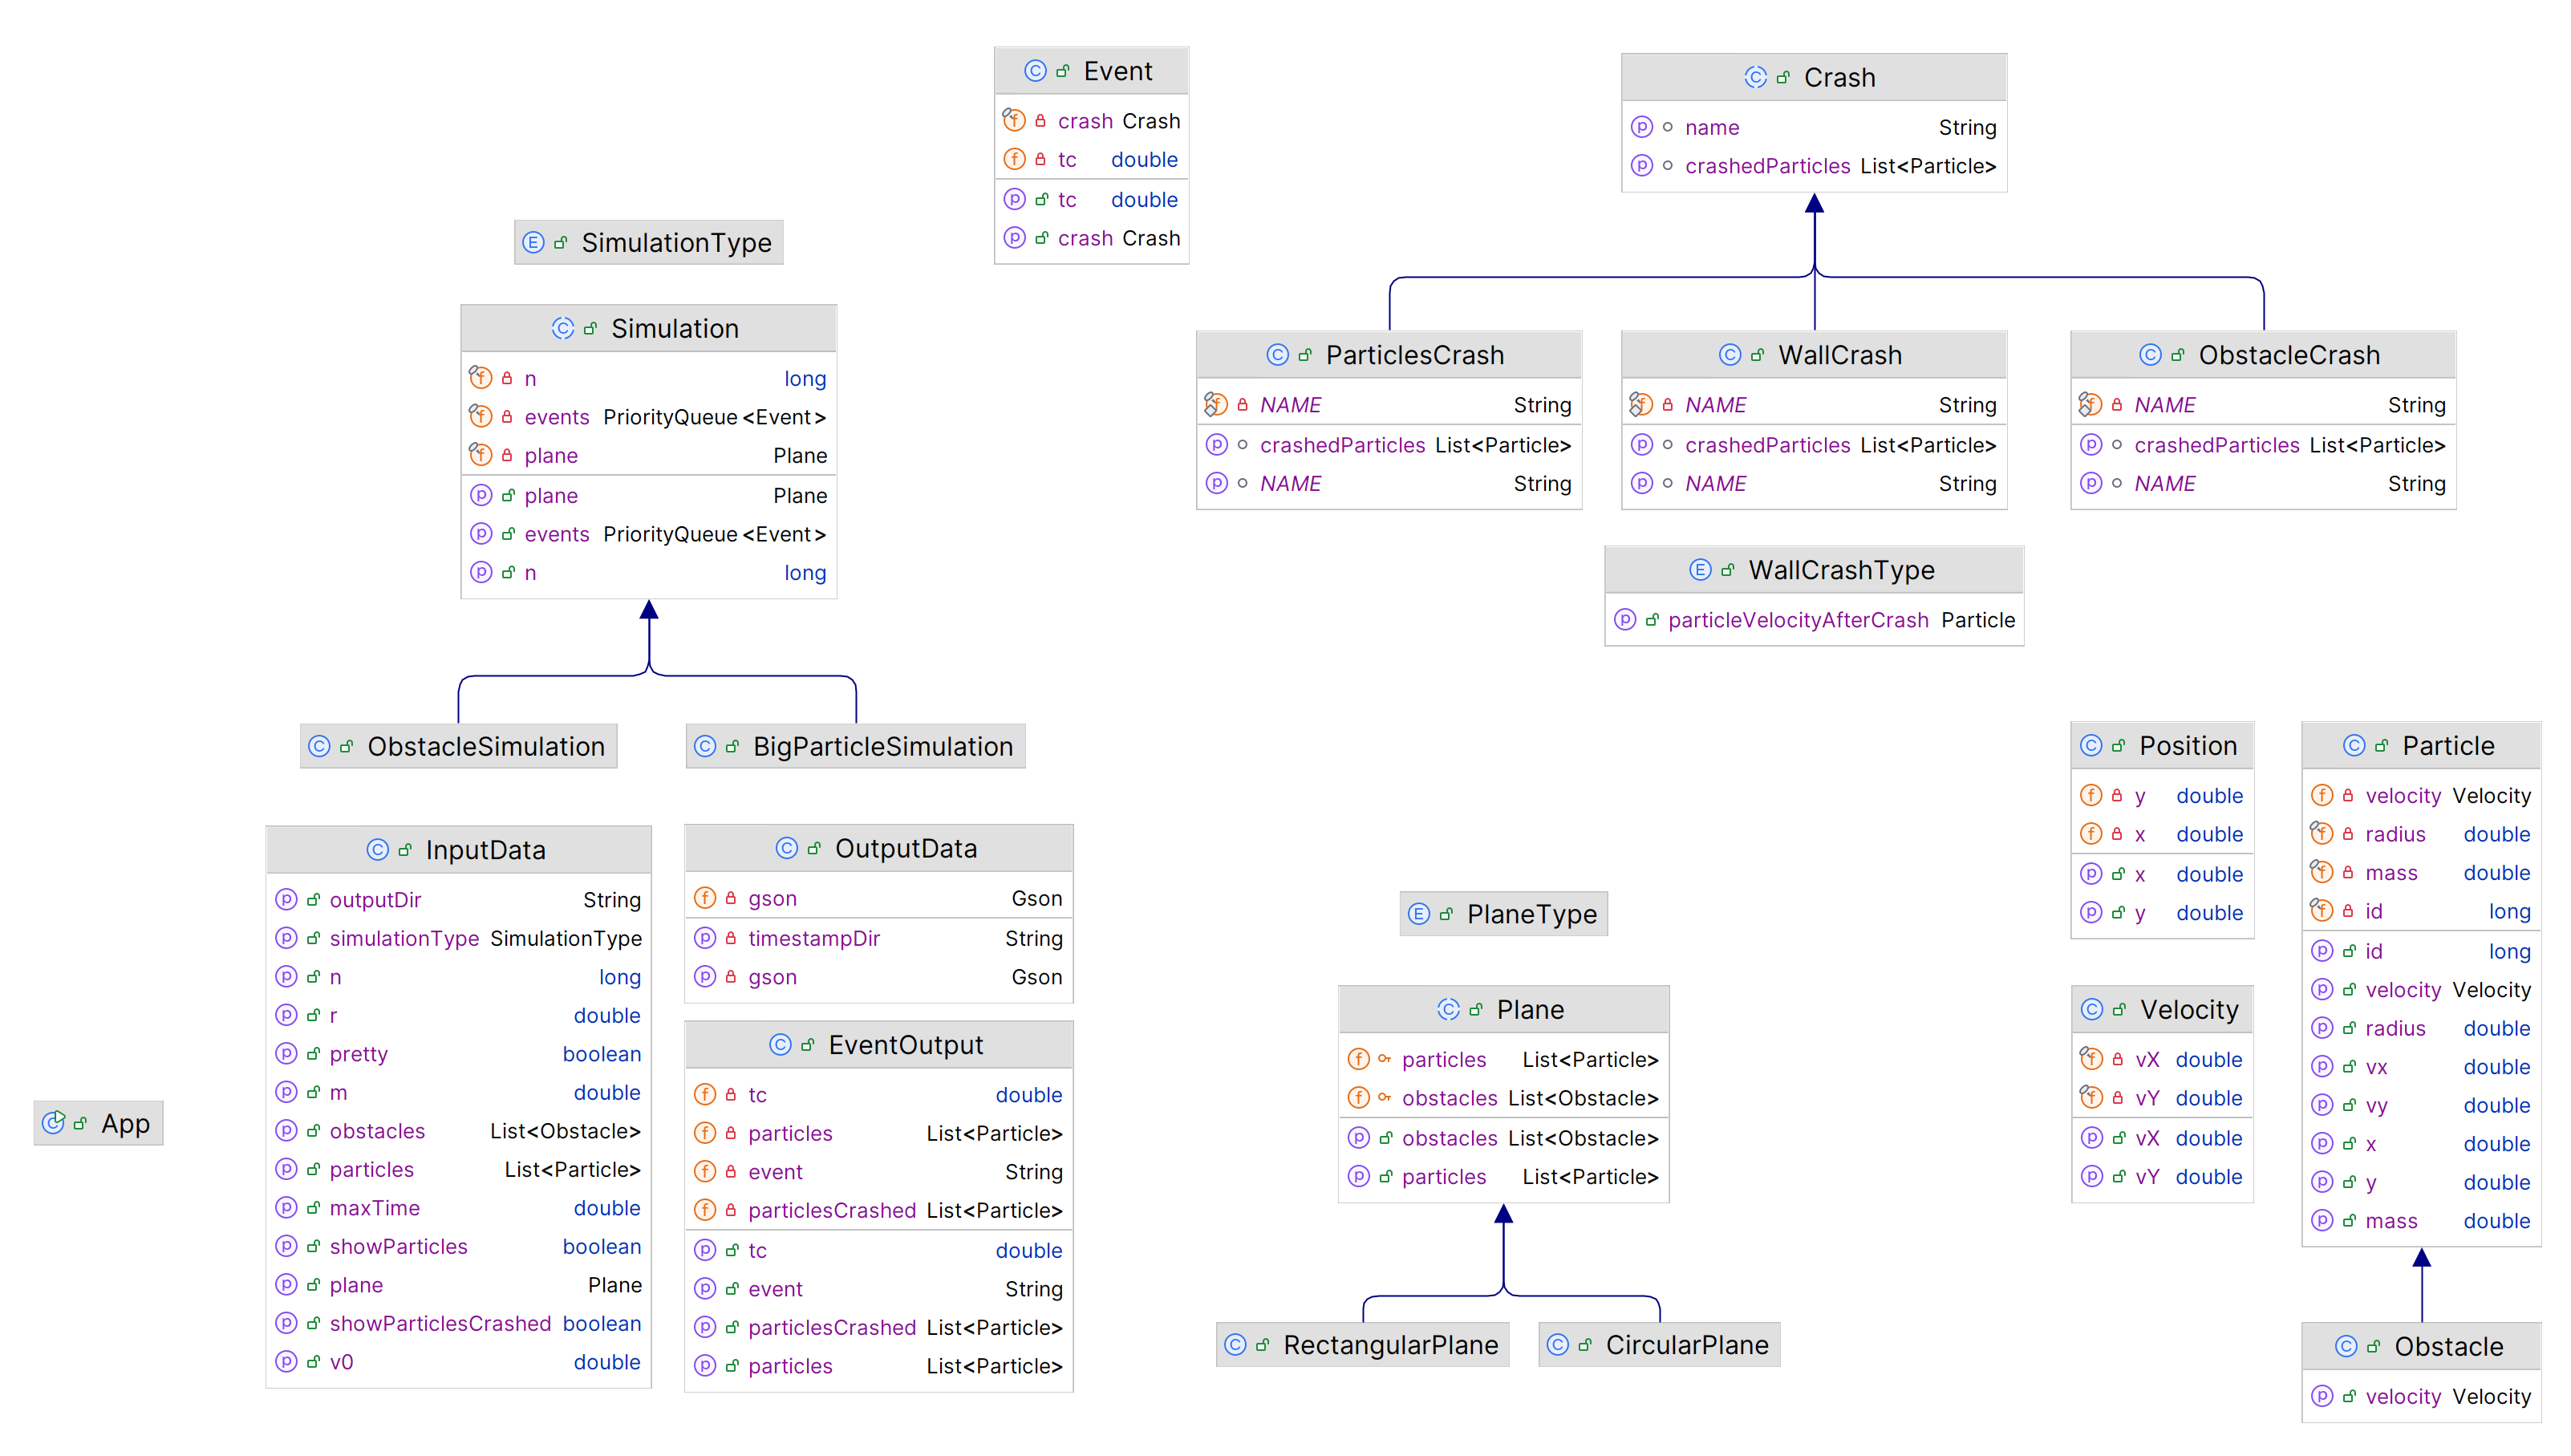
\includegraphics[width=0.6\linewidth]{UML}
    \caption{Diagrama UML}
    \label{fig:UML-Simulacion}
\end{figure}

\subsection{Simulación}\label{label:simulacion}
    La clase $LifeGame$ modela una instancia de la simulación del sistema. Por defecto, las reglas son las del juego de la vida,
    pero es posible modificar las condiciones para poder simular sistemas alternativos. Esta clase es el núcleo de la
    simulación (Ver diagrama UML~\ref{fig:UML-Simulacion}), debido a que posee todos los componentes necesarios
    para representar una instancia particular del sistema. Por su parte, $LifeGameRunner$ controlará el flujo y evolución del sistema,
    siendo invocado por $App$ que es el punto de entrada al codigo.

\subsection{Matriz de celdas}\label{subsec:matriz de celdas}
    En lo que refiere a la simulación del modelo, este ha sido diseñado para trabajar con autómatas celulares de tres
    dimensiones, ya que toda posición comprende las componentes x, y, z (Ver $Position$ en diagrama UML~\ref{fig:UML-Simulacion}).
    En caso de ser bidimensional, toda posición tomará el valor $z = 0$.

    En esta implementación se ha optado por una representación eficiente de la matriz de celdas utilizando una coleccion de
    tipo $Set$ en lugar de una estructura matricial convencional.
    La presencia de una celda en el conjunto indica que dicha celda está viva, mientras que la ausencia de la Position en
    el conjunto implica que la celda está muerta.

\subsection{Condiciones de corte}\label{label:condiciones_de_corte}
    La simulación puede finalizar por cuatro razones diferentes. Representadas como una enumeracion de JAVA, estas son:
    \begin{itemize}
        \item $BORDER$: Ocurre cuando se alcanza un paso donde existe una celda viva afuera de la matriz.
        \item $ALL\_DEAD$: Ocurre en el caso de que se alcanza un paso que no tenga celdas vivas.
        \item $MAX\_ITER$: Al alcanzar una cantidad maxima de iteraciones en la simulación. Esta cantidad es parámetro de
            entrada de la simulación.
        \item $NO\_CHANGE$: Cuando no hay variación de la matriz de celdas entre dos pasos consecutivos.
    \end{itemize}

\subsection{Código auxiliar}\label{label:codigo_aux}
    La clase $InputData$ provisiona métodos para la lectura de archivos JSON y así parametrizar la 
    simulación en función a un archivo de entrada. Por su parte, la clase OutputData exporta los 
    resultados de la simulación a un archivo JSON

    Adicionalmente, las clases $Border$, $Position$ y $NeighbourhoodCondition$ modelan el comportamiento de la matriz de
    celdas. Por otro lado, $Border$ simplemente modela las dimensiones de la matriz de celdas de la instancia particular
    del sistema a modelar. Por otro lado $Position$ es la representación de una celda dentro de la matriz.Por ultimo,
    $NeighbourhoodCondition$ es una enumeración de JAVA que implementa un método que retorna, para un determinado rango
    $r$, las celdas vecinas de una celda central según el tipo de vecindario.